\section{Backup Slides}

\begin{frame}

\centering
{\LARGE Backup Slides}

\end{frame}

\begin{frame}{Diffusion Maps Theory}

\begin{itemize}
        \item We have data $x_1, x_2, \dots, x_n \in \mathbb{R}^d$

        \item We need a {\bf distance metric} $d(x_i, x_j)$ for our data
        \item We first construct the matrix $W \in \mathbb{R}^{n \times n}$, with
        $$W_{ij} = \exp \left( -\frac{d^2 (x_i, x_j)}{\epsilon} \right) $$
        where $\epsilon$ is a characteristic distance \footcite{coifman2008graph, rohrdanz2011determination}

        \leavevmode\makebox(0,0){\put(220, 90){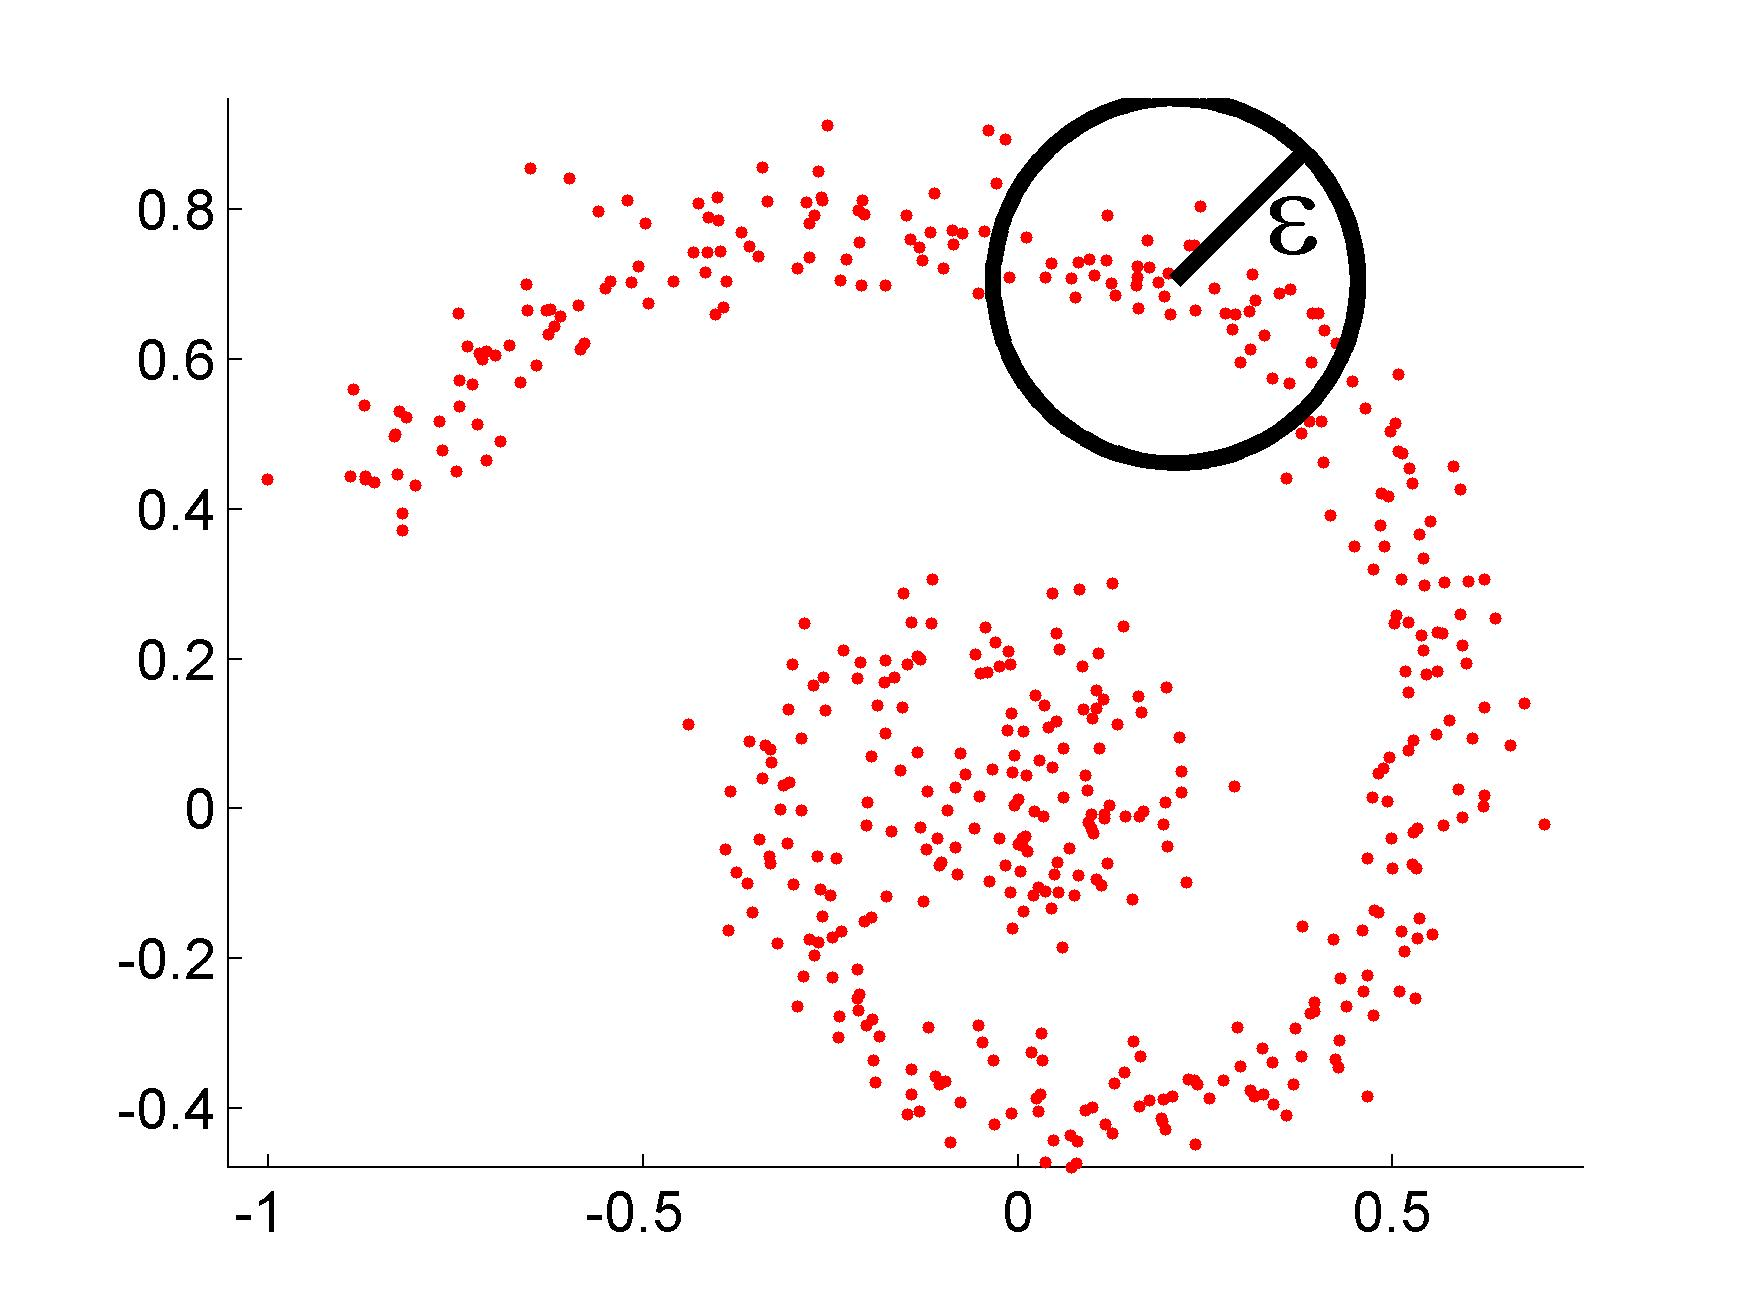
\includegraphics[width=0.3\textwidth]{spiral_with_ball}}}

        \item We define the diagonal matrix $D$ with $D_{ii} = \sum_{j=1}^{n} W_{ij}$, and $A =  D^{-1} W$, where $A$ is row-stochastic

        \item $I-A$ then approximates the Laplacian

        \item We compute the {\em real} {\bf eigenvectors} $\varphi_1, \varphi_2, \dots, \varphi_n$ and {\bf eigenvalues} $\lambda_1, \lambda_2, \dots, \lambda_n$ of $A$.

        %\item We {\bf order} the eigenvector/eigenvalue pairs such that $|\lambda_1| \ge |\lambda_2| \ge \dots \ge |\lambda_n|$

        \item The eigenvectors then approximate the eigenfunctions of the Laplacian on the manifold
    \end{itemize}
    
\end{frame}

\begin{frame}{Angular Synchronization \let\thefootnote\relax\footnote{\cite{singer2011angular}}}

    {\scriptsize
    \begin{itemize}
        \item We have data $x_1, x_2, \dots, x_n$ which is invariant under some group $G$

        \item We will take $G = SO(2)$, but other symmetry groups can also be considered

        \item Let $\theta_{ij}$ denote the angle of rotation that best aligns $x_i$ and $x_j$ (so $\theta_{ji} = -\theta_{ij}$)

        \item We seek $\hat{\theta_1}, \hat{\theta_2}, \dots, \hat{\theta_n}$ so that rotating each data point $x_i$ by $\theta_i$ will result in the most ``consistent'' aligned data

        \item We construct the matrix $H$, where $H_{ij} = e^{i \theta_{ij}}$.

        \item We then want to optimize
        $$ \max_{\theta_1, \dots, \theta_n \in [0, 2\pi)} \sum_{i=1}^{n}\sum_{j=1}^{n} e^{-i \theta_i}H_{ij} e^{i \theta_j}$$


        \item Note that if $\theta_{ij}$ is an accurate measurement, then
        $e^{-i \theta_i}H_{ij} e^{i \theta_j} = e^{-i \theta_i}e^{i (\theta_i-\theta_j)} e^{i \theta_j} = 1$

        \item However, if $\theta_{ij}$ is inaccurate, then $e^{-i \theta_i}H_{ij} e^{i \theta_j}$ will be a (uniform) random complex number of unit norm; these terms will (mostly) cancel

        \item We relax the problem to
        $$\max_{z_1, \dots, z_n \in \mathbb{C}} \sum_{i=1}^{n}\sum_{j=1}^{n} \overline{z_i} H_{ij} z_j $$
    \end{itemize}
    \par}
\end{frame}

\begin{frame}{Angular Synchronization \let\thefootnote\relax\footnote{\cite{singer2011angular}}}

    {\scriptsize
    \begin{itemize}
        \item The solution to
        $$\max_{z_1, \dots, z_n \in \mathbb{C}} \sum_{i=1}^{n}\sum_{j=1}^{n} \overline{z_i} H_{ij} z_j = \max \overline{z} H z$$
        is given by $v_1$, the top eigenvector of $H$

        \item Note that the entries of $v_1$ are not necessarily of unit norm\\
        Therefore, the optimal rotations $\hat{\theta_1}, \dots, \hat{\theta_n}$ are given by
        $e^{i \hat{\theta_i}} = \frac{v_1(i)}{|v_1(i)|}$

        \item
        Under a uniform noise model, the matrix $H$ can be shown to have an eigenvalue spectrum that consists of a semicircle distribution \footcite{wigner1955characteristic, wigner1958distribution}, with one outlier corresponding to the top eigenvector, which contains the optimal alignments\\
        \begin{center}
        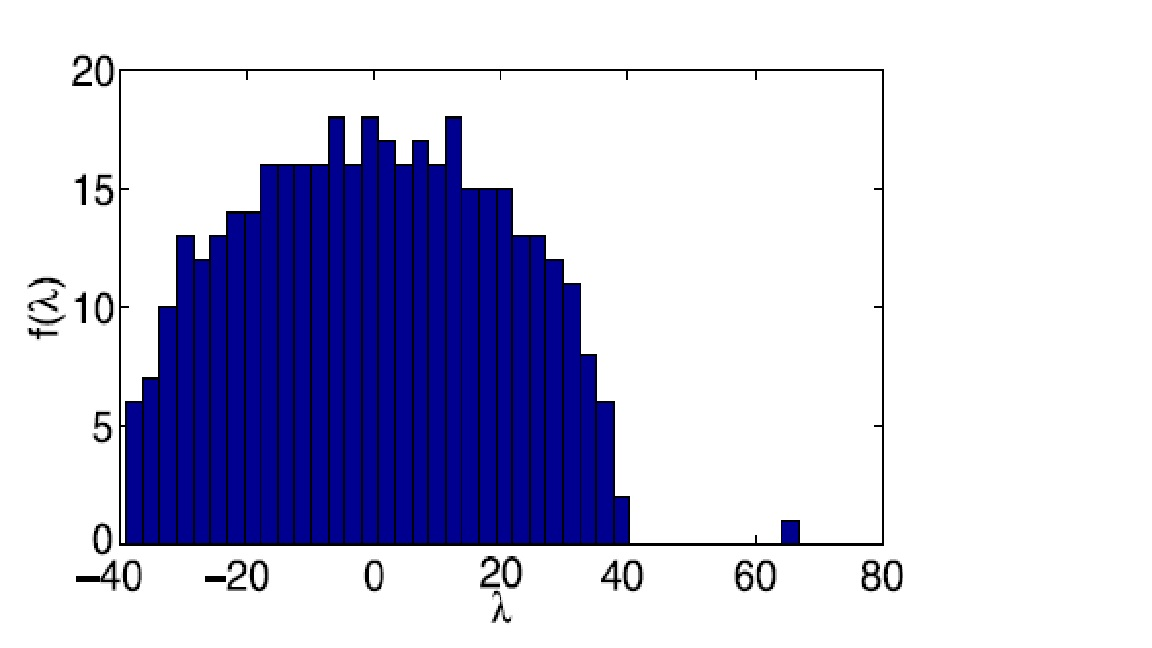
\includegraphics[width=0.3\textwidth]{evec_spectrum.jpg}
        \end{center}

        \item Also note that this formulation takes into account {\em consistency}\\
        For example, if we want to satisfy two angle relations $\theta_i-\theta_k \approx \theta_{ij} + \theta_{jk} \forall j$, we would solve
        $$\max_{z_1, \dots, z_n \in \mathbb{C}} \sum_{i=1}^{n}\sum_{k=1}^{n} \overline{z_i} \left( \sum_{j=1}^{n} e^{i (\theta_{ij} + \theta_{jk})} \right) z_k = \max \overline{z} H^2 z$$

        The solution to this optimization problem is also $v_1$, the top eigenvector of $H$
    \end{itemize}
    \par}

\end{frame}

\begin{frame}{Vector Diffusion Maps}

	\begin{itemize}
	\item We construct the matrix $W$ with
	        $$W_{ij} = \exp \left( -\frac{d^2 (x_i, x_j)}{\epsilon} \right) $$
	\item We construct the matrix $A$ with
	$$A_{ij} = \frac{W_{ij}}{\sum_j W_{ij}}$$
	
	 \item Let $\theta_{ij}$ denote the angle of rotation that best aligns $x_i$ and $x_j$ (so $\theta_{ji} = -\theta_{ij}$)

     \item We construct the matrix $H$, where $H_{ij} = e^{i \theta_{ij}}$.
     
     \item We then construct the matrix $S$, with
     $$S_{ij} = A_{ij} H_{ij}$$
     
     \item The optimal rotations are then approximated $v_1$, the top eigenvector of $S$

     \item Note that the entries of $v_1$ are not necessarily of unit norm\\
        Therefore, the optimal rotations $\hat{\theta_1}, \dots, \hat{\theta_n}$ are given by
        $e^{i \hat{\theta_i}} = \frac{v_1(i)}{|v_1(i)|}$

	\item The embedding coordinates are given by $\langle v_i(k), v_j(k) \rangle$ for all pairs $1 \le i, j \le n$
	
	\end{itemize}
\end{frame}

\begin{frame}{Translations + Rotations in VDM}

	\begin{itemize}
	
	\item Vector diffusion maps \footcite{singer2012vector} requires that the symmetry group be {\em compact}, so that the pairwise alignments are well-defined (extreme value theorem)
	\item However, the group of two--dimensional translations + rotations ($ISO(2)$) is not compact
	\item We can overcome this by mapping the group $ISO(2)$ onto the group $SO(3)$ (the space of three--dimensional rotations)
	\item We project each image onto the surface of a sphere; translations and rotations in $\mathbb{R}^2$ now correspond to {\em only} rotations of the sphere in $\mathbb{R}^3$
	\item We can now do angular synchronzation or VDM of the images projected onto a sphere, with $SO(3)$ as our symmetry group
	\end{itemize}
\end{frame}

%\begin{frame}{Scattering Transform + FT}

%\end{frame}
